\documentclass[12pt]{article}

\usepackage{natbib}
\usepackage[cm]{fullpage}
\usepackage{graphicx}
\pagenumbering{gobble}

\linespread{1.00}

\usepackage{titlesec} % Allows customization of titles

\setlength\parindent{24pt}

\usepackage[
  top    = 2.50cm,
  bottom = 1.50cm,
  left   = 1.50cm,
  right  = 1.50cm]{geometry}

\usepackage{setspace}

\title{\vspace{-25mm}\fontsize{16pt}{10pt}\selectfont\textbf{DCP: Fast Recursive Copy}} % Article title

\author{
  \textsc{William Morriss} \\
  \textsc{Thomas Kim}
}
\date{}

\begin{document}

\maketitle % Insert title

\section{Overview}
An improved version of 'cp -r,' dcp, was implemented.
This version takes advantage of Linux's asynchronous IO interfaces to create
opportunities for parallelism, and minimizes the time spent blocking on disk
IO by leveraging fallocate and readahead. In order to ensure reads
are more likely to result in hits in the buffer cache when memory is scarce, POSIX
fadvise is used. To ensure optimal layout of files for writing, POSIX
fallocate is used. The main goal of dcp is to fully saturate disk IO
at all times in order to have a fast, portable solution which supports
any POSIX compliant filesystem interface.

\section{Implementation}

\subsection{Multithreading}

\subsection{Readahead and buffer size}
POSIX fadvise is used to ensure that pages will be available
in the buffer cache when read, and that pages will be evicted from
the cache as soon as possible. All reads in dcp are
sequential, so FADV\_SEQUENTIAL is used.

Additionally, readahead is used to provide hints to the kernel
regarding the number of bytes which should be read into the buffer cache.
Currently, dcp uses a fixed-size buffer of 0x80000 bytes for reads.
As part of future work, a buffer which adaptively resizes itself based on system
load and IO speed is proposed. However, adaptively resizing the buffer introduces
some overhead and it is difficult to tune the size of the buffer for performance gains
in all workloads and across all systems. %TODO do we need this paragraph?

\subsection{Fallocate}
POSIX fallocate is used to allow the destination filesystem to
allocate blocks in an efficient way. The use of fallocate is
fairly straightforward and increases write speeds on
target ext4 and NTFS filesystems.

\section {Test platform}
\begin{tabular}{l|r r}
  Component & Specification                   & Interface \\
  CPU       & Intel i7-4770k @ 3.50ghz                    \\
  HDD A     &         1tb @ 7200rpm           & SATA 2.0  \\
  HDD B     &                 2tb @ 7200rpm   & SATA 2.0  \\
  SSD A     &         250gb                   & SATA 2.0  \\
  External A& 3tb @ 5400rpm                   & USB 3.0   \\
\end{tabular}
\section{Benchmarking methodology}
Dcp was tested on consumer-grade personal computers using 3 different types
of disk: solid state drive, traditional disk-based hard drive, and
an external USB3.0 disk based hard drive. With the exception of the external
hard drive, which is formatted in NTFS, the disks are formatted in ext4.
The combinations of stable storage media tested include:\\
\begin{tabular}{|l|l|l|}
  \hline
  source  & destination & graph label \\
  \hline
  SSD A   & SSD A       & ssd - self  \\
  SSD A   & HDD A       & ssd - hdd   \\
  SSD A   & External A  & ssd - ext   \\
  HDD A   & SSD A       & hdd - ssd   \\
  HDD A   & HDD B       & hdd - hdd   \\
  HDD A   & External A  & hdd - ext   \\
  External A & SSD A    & ext - ssd   \\
  External A & HDD A    & ext - hdd   \\
  \hline
\end{tabular} \\
Three main benchmarks were run on the data, named broad, fat, and deep.
These will be elaborated upon in the following section.

\section{Results}
Each file in the broad benchmark is 300kb (300000 bytes), and
the top level directory contains 7 files and 15 subdirectories. Each of the 15 subdirectories
contains 7 files and 15 subdirectories, which in turn contain 7 files.
The broad benchmark is % TODO, justification for why we chose this benchmark
The following graph shows the mean execution time across 5 trials of the broad benchmark across multiple disk configurations.
\vspace{5mm}

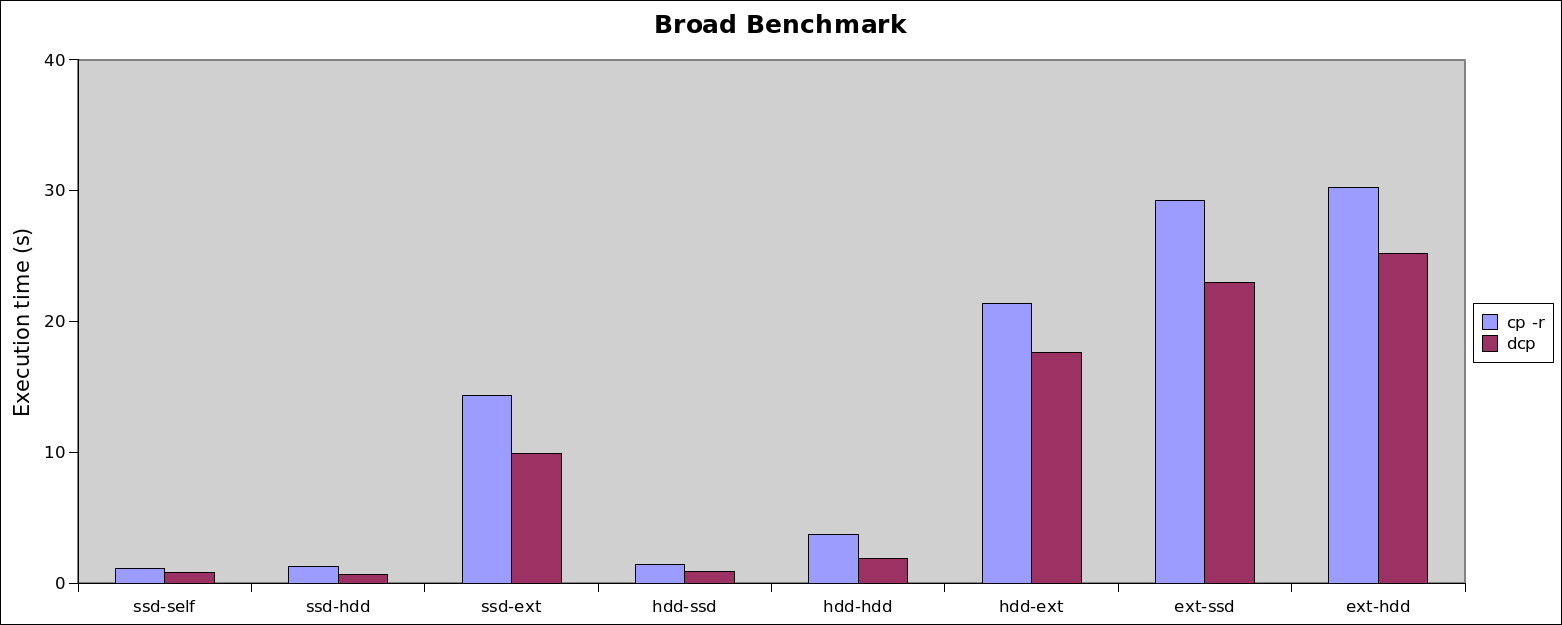
\includegraphics[width=500pt]{graphs/broad-manydisk.png}

\vspace{5mm}

The results show... %TODO

Each file in the fat benchmark is 200kb (200000 bytes), and
the top level directory contains 3 files and 35 subdirectories. Each
of the 35 subdirectories contains 3 files and 35 subdirectories, which in turn contain 3 files.
The fat benchmark is % TODO, justification for why we chose this benchmark
The following graph shows the mean execution time across 5 trials of the fat benchmark across multiple disk configurations.
\vspace{5mm}

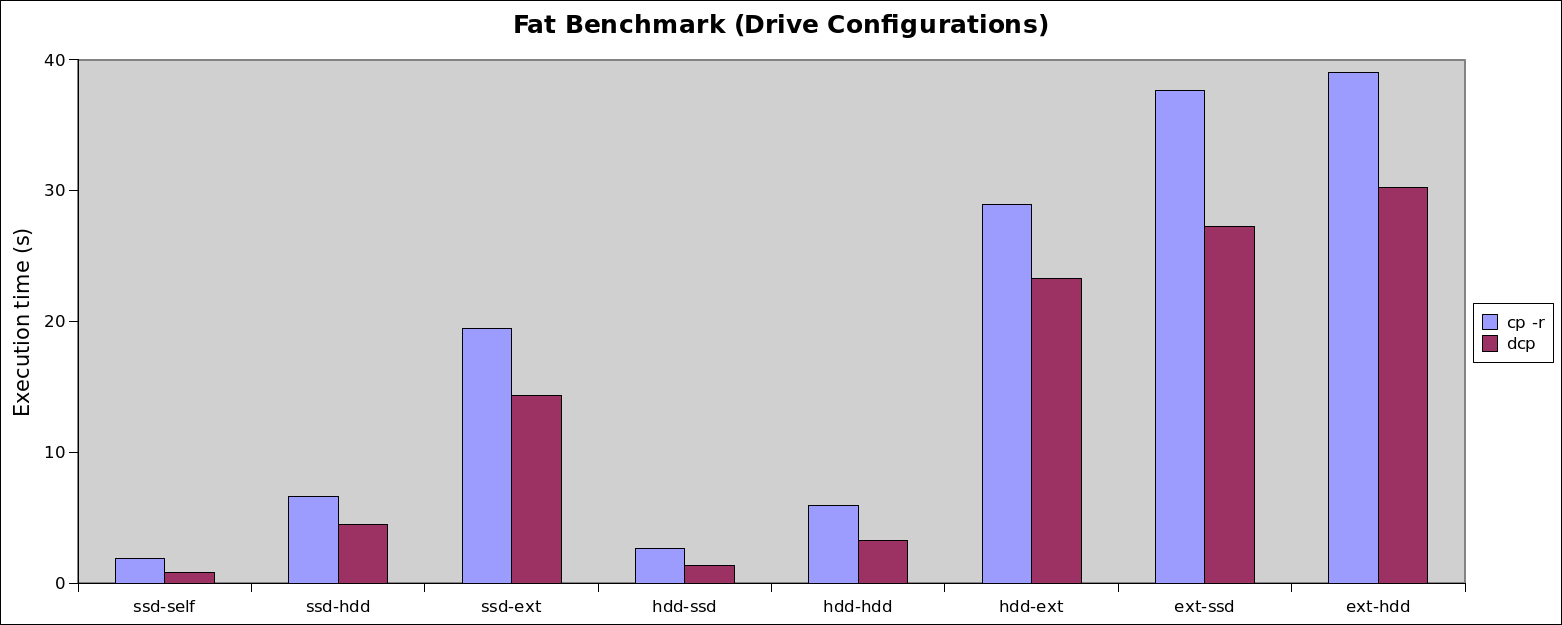
\includegraphics[width=500pt]{graphs/fat-manydisk.png}

\vspace{5mm}

Each file in the deep benchmark is 20mb (20000000 bytes), and
the top level directory contains 1 file and 1 subdirectory. There
are 6 nested subdirectories in this benchmark.
The deep benchmark is % TODO, justification for why we chose this benchmark
The following graph shows the mean execution time across 5 trials of the deep benchmark across multiple disk configurations.

\vspace{5mm}

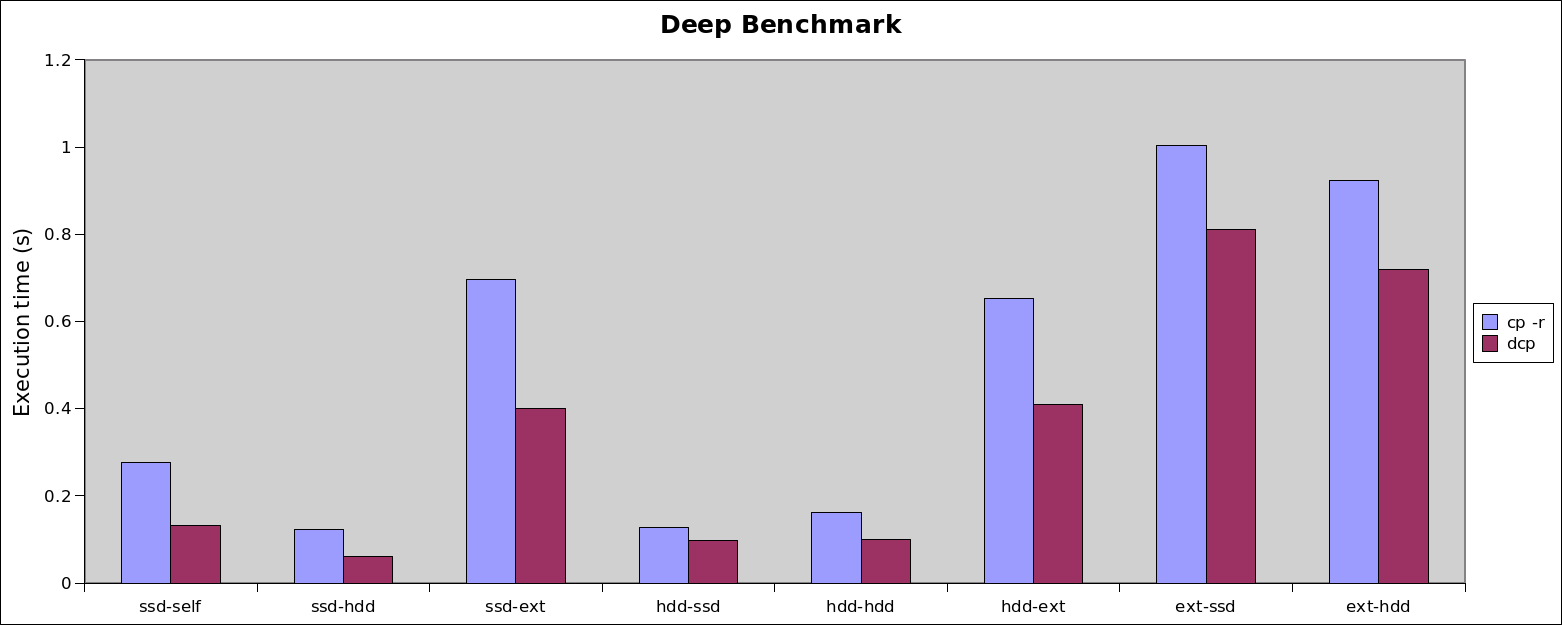
\includegraphics[width=500pt]{graphs/deep-manydisk.png}

\vspace{5mm}

\section{Practical test}
Additionally, one practical test was done to demonstrate the advantage
of dcp over standard cp -r. 5.7gb of video files split among 5 subdirectories were copied between
HDD A and HDD B to simulate a backup of videos, a usage pattern common for one of the researchers.
This benchmark was not repeated for other drive types as it is simply intended to convey a practical example use
case.

The results on this practical test show that dcp in its current state outperforms cp -r by a decent margin even
in situations where a disk's theoretical maximum throughput is approached (typically with large sequential reads/writes).
The mean execution time of cp -r is approximately 2:10, while the mean execution time of dcp is 1:50, with a sample standard deviation of
5 seconds and $p < 0.01$.



\end{document}
